\documentclass[11pt, oneside]{article}   	% use "amsart" instead of "article" for AMSLaTeX format
\usepackage{geometry}                		% See geometry.pdf to learn the layout options. There are lots.
\geometry{letterpaper}                   		% ... or a4paper or a5paper or ... 
%\geometry{landscape}                		% Activate for for rotated page geometry
%\usepackage[parfill]{parskip}    		% Activate to begin paragraphs with an empty line rather than an indent
\usepackage{graphicx}				% Use pdf, png, jpg, or eps� with pdflatex; use eps in DVI mode
								% TeX will automatically convert eps --> pdf in pdflatex		
\usepackage{amssymb}
\usepackage{amsmath}
\usepackage{parskip}
\usepackage{color}
\usepackage{hyperref}

\title{Cauchy integral theorem}
%\author{The Author}
%\section{}
%\subsection*{}
\date{}							% Activate to display a given date or no date

\graphicspath{{/Users/telliott_admin/Dropbox/Tex/png/}}
% \begin{center} 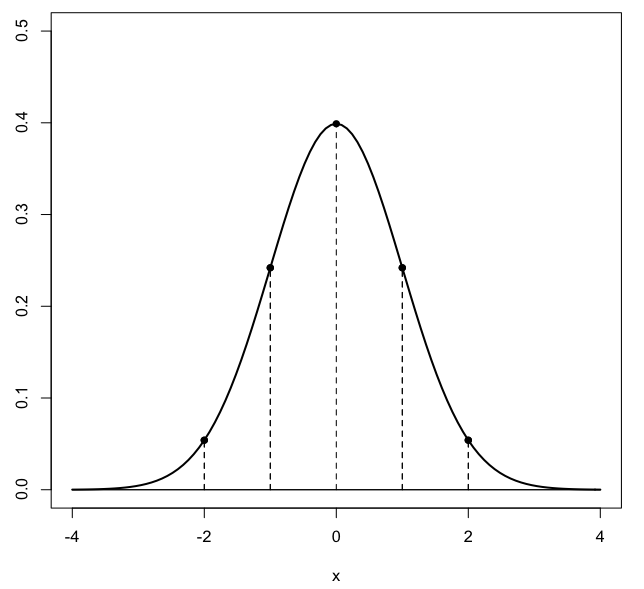
\includegraphics [scale=0.4] {gauss3.png} \end{center}
\begin{document}
\maketitle
\Large

\subsection*{Cauchy' First Integral Theorem}

Cauchy 1 is a theorem that says the integral of an analytic function over a closed path (over a region without a singularity), is equal to zero.
\[ \oint_C f(z) \ dz = 0 \]
We proved this in the last part, so ssume that the theorem is correct.  

We will integrate the function $f(z) = z$ over a rectangle ($R = [0,a] \times [b,0]$.  Write
\[ z = x + i y \]
\[ dz = dx + i dy \]
\[ f(x,y) = u(x,y) + iv(x,y) \]
Our integral is
\[ \int z \ dz = \int (u + iv) \ (dx + i dy) \]
\[ = \int u \ dx - \int v \ dy + i \int v \ dx + i \int u \ dy \]
Since the whole thing is equal to zero over our closed path, both parts are equal to zero:
\[ \int u \ dx - \int v \ dy = 0 \]
\[ \int v \ dx + \int u \ dy \]
Does this look familiar??

\subsection*{application of Cauchy 1}

The function we'll be working with is the one we introduced before:
\[ u(x,y) =  e^{-x^2} e^{y^2} \cos 2xy \]
\[ v(x,y) = e^{-x^2} e^{y^2} (- \sin 2xy) \]
Everything will simplify pretty quickly.  Divide the path into its four parts and compute each separately:
Over $C1$, $y=0$ and $dy = 0$ so we have:
\[ \int_{C1} = \int u \ dx = \int_0^a e^{-x^2} e^{0} \cos 0 \ dx = \int_0^a e^{-x^2} \ dx \]
C2 ($x = a$, $dx = 0)$:
\[ \int_{C2} = - \int_0^b e^{-a^2} e^{y^2} (- \sin 2ay) \ dy  \]
C3 ($y = a$, $dy = 0)$:
\[ \int_{C3} = \int_a^0 e^{-x^2} e^{b^2} (\cos 2bx) \ dx  \]
C4 ($x = 0$, $dx = 0$):
\[ \int_{C4} = \int_b^0 e^{y^2} (-\sin 0) \ dy = 0 \]
So all together:
\[ \int_0^a e^{-x^2} \ dx - \int_0^b e^{-a^2} e^{y^2} (- \sin 2ay) \ dy + \int_a^0 e^{-x^2} e^{b^2} \cos 2bx \ dx = 0 \]
\[ \int_0^a e^{-x^2} \ dx = e^{-a^2} \int_0^b e^{y^2} (- \sin 2ay) \ dy + e^{b^2} \int_0^a e^{-x^2} \cos 2bx \ dx  \]
Let $a \rightarrow \infty$.  Then
\[ e^{-a^2} \rightarrow 0 \]
so the first term on the right side goes to zero and we have:
\[ \int_0^{\infty} e^{-x^2} \ dx = e^{b^2} \int_0^{\infty} e^{-x^2} \cos 2bx \ dx  \]
But we know the value of the left-hand side, it is 
\[ \int_0^{\infty} e^{-x^2} \ dx = \frac{\sqrt{\pi}}{2} \]
so
\[  \int_0^{\infty} e^{-x^2} \cos 2bx \ dx = \frac{\sqrt{\pi}}{2} \ e^{-b^2} \]
The Gaussian that we knew, is a special case of this general form.

\end{document}  